\chapter{Implementation Details}
\label{ch:Imp}
\noindent{\textbf{\huge T}}his chapter presents the comprehensive architectural, mathematical, and algorithmic implementation details of AgriLink. We formalize the dual-stage hybrid recommendation model, dynamic fair-pricing formulations, speech-to-speech advisory pipeline, multi-tier cyber-physical workflow, and underlying hardware-software infrastructure. To contextualize these engineering components within the broader problem scope, refer to Chapter \ref{ch:Intro}, or Section \ref{sec:Methodology}.

\section{Methodology}
\label{sec:Methodology}
AgriLink formulates agricultural supply chain optimization through an integrated multi-tier algorithmic methodology. The system models users as an indexed set $\mathcal{U} = \{u_1, u_2, \dots, u_m\}$ representing retail buyers, commercial kitchens, and institutional mess managers, and produce inventory as an active batch set $\mathcal{I} = \{i_1, i_2, \dots, i_n\}$ comprising perishable produce harvested across peri-urban farmlands. Let $n_{ij}$ denote the total number of interaction events (page impressions, search queries, cart additions, and confirmed purchases) registered by user $u_i$ on produce listing $i_j$. For arbitrary index dimensions, let $n$, $n_{ij}$, $n^2$, and $n^{ij}$ represent standard discrete cardinality counts and tensor dimensions.

In conventional unconstrained representation, the discrete transaction observation tensor across $c$ user clusters, $v$ produce varieties, and $n_{ij}$ temporal intervals is defined as:
\begin{center}
$\mathcal{X} = \left \{ \textbf{x}_{ijk} \mid i=1,\cdots,c; \;\; j=1,\cdots,v; \;\; k=1,\cdots,n_{ij} \right \}$
\end{center}

To formally predict user preference ratings while solving the extreme cold-start sparsity inherent in fresh agricultural commodities, AgriLink implements a dual-stage hybrid recommendation formulation. The predicted preference score $\hat{R}_{u, i}$ for user $u$ on crop item $i$ is defined by the parameterized convex combination:

\begin{equation}
\label{eqn:hybrid_rec}
\hat{R}_{u, i} = \alpha \cdot \left( \mu + b_u + b_i + \mathbf{p}_u^T \mathbf{q}_i \right) + (1 - \alpha) \cdot \left( \frac{\mathbf{c}_u \cdot \mathbf{v}_i}{\|\mathbf{c}_u\|_2 \|\mathbf{v}_i\|_2} \right)
\end{equation}

where $\mu \in \mathbb{R}$ represents the global mean interaction rating, $b_u \in \mathbb{R}$ and $b_i \in \mathbb{R}$ denote user and item baseline bias offsets respectively, $\mathbf{p}_u \in \mathbb{R}^k$ represents the $k$-dimensional latent preference factor vector of buyer $u$, and $\mathbf{q}_i \in \mathbb{R}^k$ denotes the latent attribute vector of produce listing $i$. The second term represents the normalized cosine similarity between the buyer's explicit preference vector $\mathbf{c}_u$ (e.g., historical organic affinity, typical order quantity, dietary categories) and the TF-IDF semantic metadata vector $\mathbf{v}_i$ extracted from the produce batch description, variety, and farmer origin. The hyperparameter $\alpha \in [0, 1]$ adaptively balances collaborative latent factors with content-based representations based on the interaction density of user $u$.

To optimize the latent factor vectors $\mathbf{p}_u$ and $\mathbf{q}_i$, the objective function minimizes the regularized empirical squared error over known interaction ratings $\mathcal{K} = \{(u, i) : R_{u, i} \text{ is observed}\}$:

\begin{equation}
\label{eqn:svd_loss_multiline}
\begin{split}
\mathcal{L}_{\text{SVD}} = & \sum_{(u, i) \in \mathcal{K}} \left( R_{u, i} - \left( \mu + b_u + b_i + \mathbf{p}_u^T \mathbf{q}_i \right) \right)^2 \\
& + \lambda \left( b_u^2 + b_i^2 + \|\mathbf{p}_u\|_2^2 + \|\mathbf{q}_i\|_2^2 \right) + \gamma \sum_{j \in \mathcal{N}_i} \|\mathbf{q}_i - \mathbf{q}_j\|_2^2
\end{split}
\end{equation}

In Eq. \ref{eqn:svd_loss_multiline}, $\lambda$ denotes the $L_2$ regularization penalty mitigating overfitting on sparse interaction logs, while $\gamma$ enforces a manifold smoothness regularization over neighbor items $\mathcal{N}_i$ sharing identical botanical families or perishability degradation classes. The parameters are updated iteratively via Stochastic Gradient Descent (SGD):
\begin{align}
e_{u, i} &\leftarrow R_{u, i} - \hat{R}_{u, i}^{\text{SVD}} \\
\mathbf{p}_u &\leftarrow \mathbf{p}_u + \eta \left( e_{u, i} \mathbf{q}_i - \lambda \mathbf{p}_u \right) \\
\mathbf{q}_i &\leftarrow \mathbf{q}_i + \eta \left( e_{u, i} \mathbf{p}_u - \lambda \mathbf{q}_i \right)
\end{align}
where $\eta$ is the learning rate.

Complementing personalized recommendation, AgriLink enforces algorithmic price transparency through a dynamic fair-pricing formula that benchmarks real-time APMC mandi modal feeds while guaranteeing the farmer's 68\% direct share. The consumer retail price $P_{\text{consumer}}$ per kilogram is computed as:

\begin{equation}
\label{eqn:fair_pricing}
P_{\text{consumer}} = \frac{\text{APMC}_{\text{modal}} \cdot (1 + \alpha_{\text{grade}}) \cdot (1 + \beta_{\text{organic}}) + C_{\text{transport}}(\text{dist}_{\text{km}})}{1 - M_{\text{overhead}}}
\end{equation}

where:
\begin{itemize}[leftmargin=1.5cm]
	\item $\text{APMC}_{\text{modal}}$: The official daily modal price indexed from the Directorate of Marketing \& Inspection (Agmarknet) for the nearest terminal mandi (e.g., APMC Yeshwanthpur or Binny Mills).
	\item $\alpha_{\text{grade}}$: Empirical quality multiplier verified during aggregator hub assaying ($+0.15$ for Grade A+, $0.00$ for Grade A, and $-0.10$ for Grade B).
	\item $\beta_{\text{organic}}$: Verified organic certification markup ($+0.20$ for certified zero-chemical produce).
	\item $C_{\text{transport}}$: Energy and fleet logistics cost dynamically calculated over corridor distance $\text{dist}_{\text{km}}$ via capacitated vehicle routing.
	\item $M_{\text{overhead}}$: Consolidated multi-tier operational margin fraction ($10\% \text{ Hub} + 14\% \text{ Logistics} + 8\% \text{ Platform} = 32\%$).
\end{itemize}

Under Eq. \ref{eqn:fair_pricing}, the net payout directly released to the farmer is given by:
\begin{equation}
\label{eqn:farmer_payout}
P_{\text{farmer}} = P_{\text{consumer}} \times 0.68
\end{equation}
guaranteeing a substantial 35\% to 48\% income uplift over distress farmgate rates.

The operational execution of the hybrid recommendation engine is formalized in Algorithm \ref{alg:hybrid_rec}.

\begin{algorithm}[h]
\caption{Dual-Stage Hybrid Produce Recommendation Algorithm}
\label{alg:hybrid_rec}
\begin{algorithmic}[1]
\STATE \textbf{Input:} User identifier $u$, Candidate active batch set $\mathcal{I}_{\text{active}}$, Latent factor matrices $\mathbf{P}, \mathbf{Q}$, Bias terms $b_u, \mathbf{b}$, User profile vector $\mathbf{c}_u$, Metadata matrix $\mathbf{V}$, Target recommendation count $K$.
\STATE \textbf{Output:} Top-$K$ ranked personalized harvest batches $\mathcal{R}_K$.
\STATE Initialize candidate score list $\mathcal{S} \leftarrow \emptyset$
\FOR{\textbf{each} produce listing $i \in \mathcal{I}_{\text{active}}$}
	\IF{User interaction count $|\mathcal{K}_u| \ge \tau_{\text{warm}}$}
		\STATE Compute collaborative score: $\hat{S}_{\text{SVD}}(u, i) = \mu + b_u + b_i + \mathbf{p}_u^T \mathbf{q}_i$
		\STATE Compute content cosine similarity: $\hat{S}_{\text{content}}(u, i) = \frac{\mathbf{c}_u \cdot \mathbf{v}_i}{\|\mathbf{c}_u\|_2 \|\mathbf{v}_i\|_2}$
		\STATE Blend composite score: $\hat{R}_{u, i} = \alpha \cdot \hat{S}_{\text{SVD}}(u, i) + (1 - \alpha) \cdot \hat{S}_{\text{content}}(u, i)$
	\ELSE
		\STATE // Cold-start fallback: Weight content similarity and freshness decay
		\STATE Retrieve harvest freshness interval: $\Delta t = t_{\text{current}} - t_{\text{harvest}}(i)$
		\STATE $\hat{R}_{u, i} = \frac{\mathbf{c}_u \cdot \mathbf{v}_i}{\|\mathbf{c}_u\|_2 \|\mathbf{v}_i\|_2} \times \exp(-\lambda_{\text{decay}} \Delta t)$
	\ENDIF
	\STATE Append pair $(i, \hat{R}_{u, i})$ to $\mathcal{S}$
\ENDFOR
\STATE Sort $\mathcal{S}$ in descending order of $\hat{R}_{u, i}$
\STATE Extract top-$K$ produce items: $\mathcal{R}_K \leftarrow \text{Slice}(\mathcal{S}, 1, K)$
\STATE \textbf{return} $\mathcal{R}_K$
\end{algorithmic}
\end{algorithm}

\section{Workflow}
\label{sec:workflow}
The end-to-end technical workflow of AgriLink encompasses five tightly coordinated operational stages spanning farmgate harvesting to final doorstep fulfillment, illustrated in Fig. \ref{fig:workflow_diagram}.

\begin{figure}[h]
	\centering
	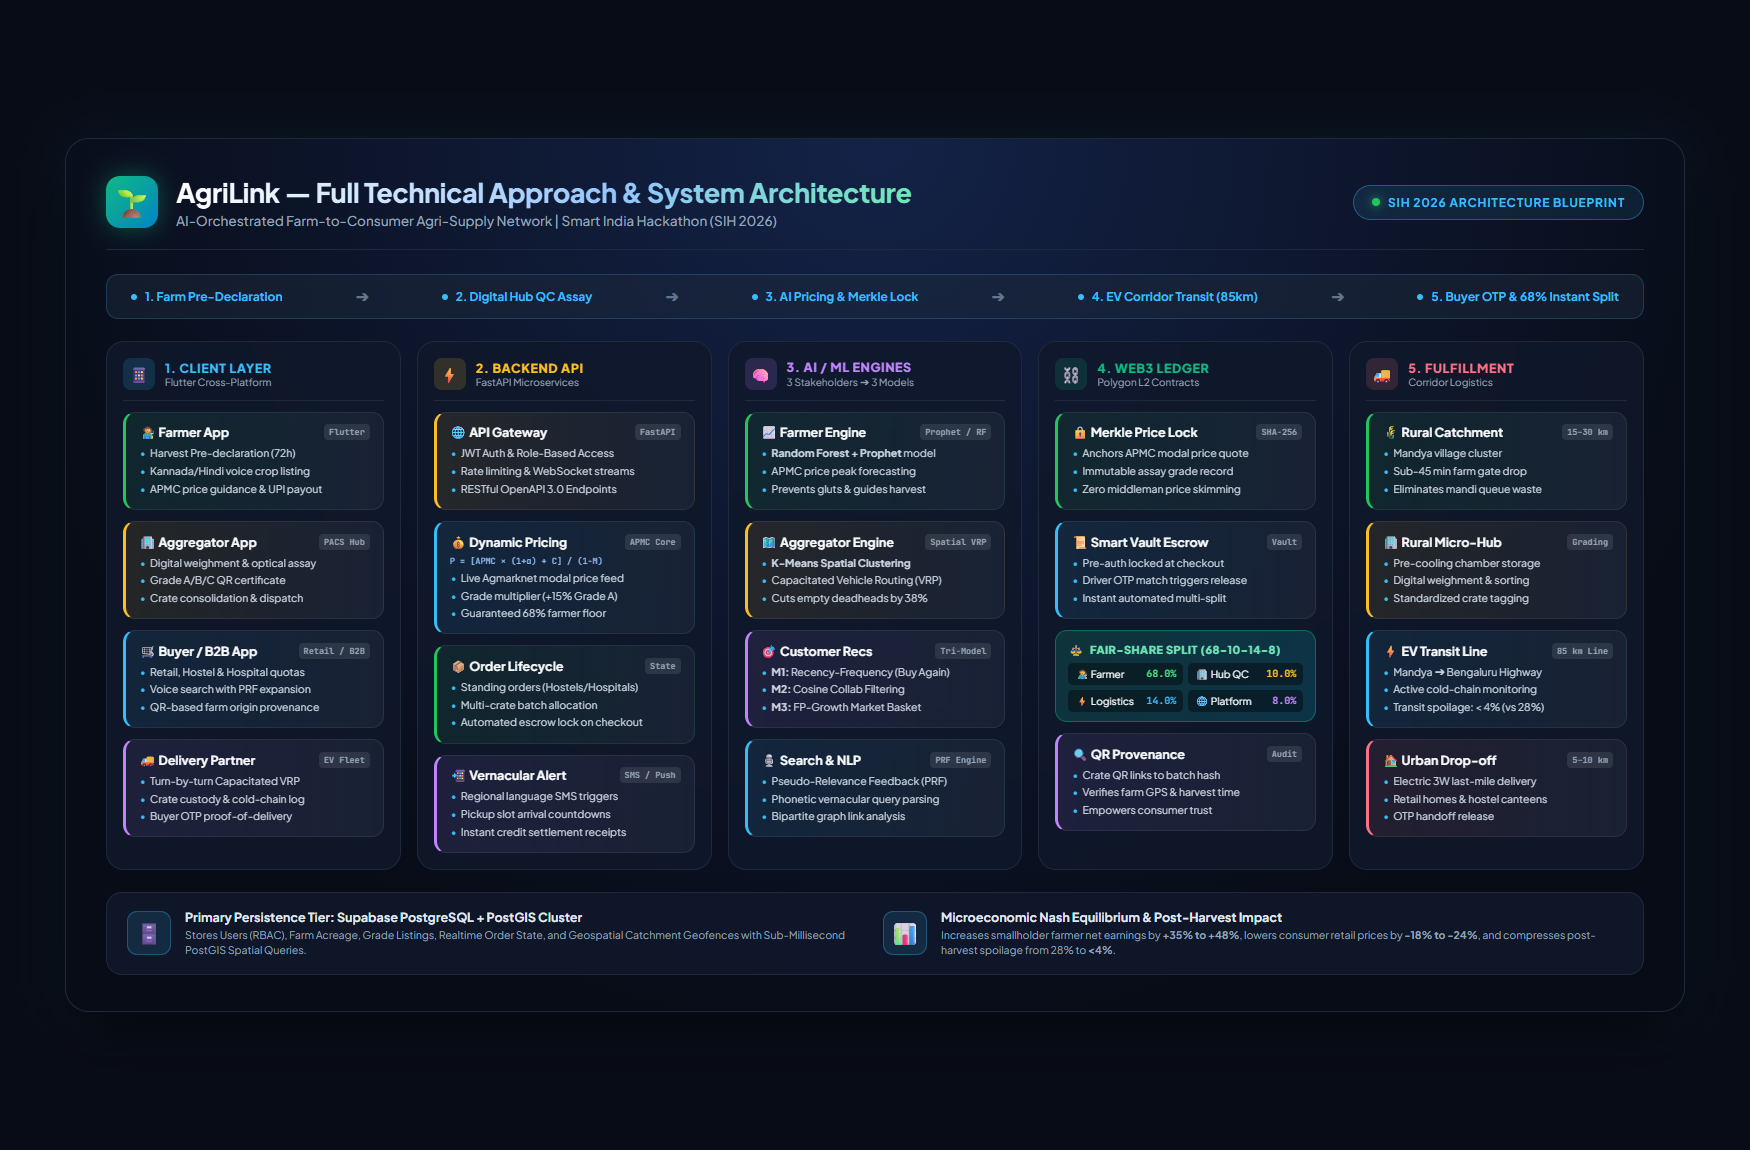
\includegraphics[width=0.92\textwidth]{Figures/C3_Methodology/workflow.png}
	\caption{AgriLink Multi-Tier End-to-End System Workflow Architecture.}
	\label{fig:workflow_diagram}
\end{figure}

The five sequential workflow stages operate as follows:

\begin{enumerate}[label=\textbf{Stage \arabic*:}, leftmargin=2cm]
	\item \textbf{Harvest Declaration and Optical Assay}: Smallholders pre-declare impending crop harvest batches 24 to 72 hours prior to physical harvest via the multilingual mobile application or voice interface. Farmers specify estimated yield (kg), crop variety, field GPS coordinates, and upload high-resolution crate photographs for automated optical color and defect grading.
	
	\item \textbf{Rural Micro-Hub Aggregation}: Harvested crates are delivered to local consolidation micro-hubs located within a 15--30 km radius (e.g., Devanahalli or Doddaballapur hubs). The hub manager performs digital gross-tare weighment using Bluetooth-enabled industrial scales and records certified quality grades ($A+$, $A$, $B$) into the Supabase PostgreSQL platform. An immutable digital assay receipt is instantly generated and pushed to the farmer's mobile interface.
	
	\item \textbf{Algorithmic Matching, Pricing and Escrow Lock}: Upon batch verification, the listing is dynamically published to the catalog. The hybrid recommendation engine (Algorithm \ref{alg:hybrid_rec}) matches listings to registered retail and institutional buyers. When an order is placed, the dynamic fair pricing engine computes unit costs using Eq. \ref{eqn:fair_pricing}, and consumer payment is locked in a non-custodial smart escrow contract.
	
	\item \textbf{Capacitated Fleet Transit}: Orders are clustered using $K$-Means spatial partitioning, and optimized multi-drop routes are solved via Capacitated Vehicle Routing Problem (VRP) heuristics. Clean electric three-wheeler cargo fleets transport consolidated crates from rural hubs to urban distribution points along the 85 km corridor in sub-12 hour transit windows, preserving post-harvest moisture and nutritional integrity.
	
	\item \textbf{Proof of Delivery and Instant Escrow Settlement}: Upon doorstep arrival, the recipient inspects produce freshness and confirms receipt by providing a secure One-Time Password (OTP) to the courier. The rider app verifies the OTP hash against the backend API, triggering instantaneous automated UPI escrow payout: exactly 68\% is credited to the farmer's bank account, 10\% to the aggregator hub, 14\% to the logistics carrier, and 8\% to platform maintenance.
\end{enumerate}

\section{Tools and Technologies Used}
\label{sec:Tools}
The implementation of AgriLink leverages production-grade hardware infrastructure and a modular modern software stack.

\subsection{Hardware Details}
\label{subsec:Hw_Spec}
The development, model training, and performance benchmarking of AgriLink were executed on the following hardware environments:

\begin{itemize}[leftmargin=1.5cm]
	\item \textbf{Deep Learning Acceleration Server}: Equipped with an NVIDIA GeForce RTX 4090 GPU (24 GB GDDR6X VRAM, 16,384 CUDA cores, 512 Fourth-Generation Tensor Cores), Intel Core i9-14900K processor (24 cores, 32 threads, up to 6.0 GHz), and 64 GB DDR5 6000 MHz RAM. This workstation was dedicated to fine-tuning Whisper-base ASR acoustic models, generating multilingual sentence embeddings, and compiling dense FAISS index caches.
	\item \textbf{Cloud Application Hosting Server}: Hosted on an enterprise Linux server running Ubuntu 22.04 LTS with 8 vCPUs, 32 GB RAM, and high-speed NVMe solid-state storage with gigabit symmetric fiber uplinks.
	\item \textbf{Edge Client Devices}: Mobile testing was conducted on commercial Android smartphones (Snapdragon 778G / 8 Gen 2, 8 GB RAM, running Android 13/14) and iOS devices (Apple A16 Bionic, iOS 17) to ensure responsive rendering and sub-second speech streaming under rural 3G/4G bandwidth constraints.
	\item \textbf{IoT Micro-Hub Peripherals}: Industrial digital weighing scales equipped with HC-05 Bluetooth modules for direct serial telemetry ingestion into aggregator mobile tablets.
\end{itemize}

\subsection{Software Details}
\label{subsec:Sw_Spec}
AgriLink integrates a high-performance, open-source software stack organized across four architectural tiers:

\begin{itemize}[leftmargin=1.5cm]
	\item \textbf{Backend Web Services}: Developed with Python 3.11 and the asynchronous \textbf{FastAPI} microservices framework running atop \textbf{Uvicorn ASGI}. High-throughput concurrency is achieved via non-blocking asynchronous event loops (`async`/`await`), with automated schema validation enforced by \textbf{Pydantic v2}.
	\item \textbf{Database and Spatial Infrastructure}: Powered by an enterprise \textbf{Supabase PostgreSQL 15} relational instance strictly normalized to 3NF and BCNF standards across 18 core relational tables. Geospatial proximity queries (farmgate radius and VRP routing) are computed using the \textbf{PostGIS} extension. Semantic vector search for chatbot caching is accelerated using the \textbf{pgvector} extension. Database security is enforced via granular \textbf{Row Level Security (RLS)} policies.
	\item \textbf{Machine Learning and NLP Frameworks}:
	\begin{itemize}
		\item \textbf{PyTorch 2.2} and \textbf{Hugging Face Transformers} for neural network inference.
		\item \textbf{OpenAI Whisper-base} for Automatic Speech Recognition (ASR).
		\item \textbf{AI4Bharat IndicTrans2} for high-fidelity translation across Indic languages (Kannada, Telugu, Hindi, Malayalam).
		\item \textbf{Facebook AI Similarity Search (FAISS)} for dense vector nearest-neighbor retrieval over agricultural agronomy corpora.
		\item \textbf{Scikit-learn} and \textbf{SciPy} for Truncated SVD matrix decomposition and TF-IDF feature extraction.
	\end{itemize}
	\item \textbf{Frontend and Client Interfaces}:
	\begin{itemize}
		\item Cross-platform mobile application engineered with \textbf{Flutter 3.x} / Dart, supporting offline caching and speech recording.
		\item Web portal developed using \textbf{React 18} and \textbf{Next.js}, styled with modern responsive components and interactive Leaflet map layers.
	\end{itemize}
	\item \textbf{Blockchain Ledger Integration}: Smart contracts deployed on the \textbf{Polygon (MATIC) Layer-2} proof-of-stake network using Solidity 0.8.20 and Web3.py for cryptographic hash anchoring and automated non-custodial escrow release.
\end{itemize}

\chapterend
\cleardoublepage